% This is samplepaper.tex, a sample chapter demonstrating the
% LLNCS macro package for Springer Computer Science proceedings;
% Version 2.20 of 2017/10/04
%
\documentclass[runningheads]{llncs}
%
\usepackage{graphicx}
\usepackage{url}
\usepackage{graphicx}
\usepackage{multirow}
\usepackage{listings}
\usepackage[table,xcdraw]{xcolor}
\usepackage{pdfpages}
% Used for displaying a sample figure. If possible, figure files should
% be included in EPS format.
%
% If you use the hyperref package, please uncomment the following line
% to display URLs in blue roman font according to Springer's eBook style:
% \renewcommand\UrlFont{\color{blue}\rmfamily}

\begin{document}
%
\title{Benchmarking databases focusing on small to medium sized personal projects 
\thanks{Supported by Institut für Information Systems Engineering (E194) Compilers and Languages (E194-5)  and written for the course "Forschungsmethoden SS20 (Research methods)"}}
%
%\titlerunning{Abbreviated paper title}
% If the paper title is too long for the running head, you can set
% an abbreviated paper title here
%
\author{Florian Nemling\inst{1} \and Renad Quku\inst{1} }
%
\authorrunning{Nemling and Quku}
% First names are abbreviated in the running head.
% If there are more than two authors, 'et al.' is used.
%
\institute{Vienna University of Technology, Karlsplatz 1040 Wien, Austria}
%
\maketitle              % typeset the header of the contribution
%
\begin{abstract}
Persistent storages are a very efficient way to save our data. In this paper we want to compare three very well-known Relational Database Management Systems: MySQL, PostgreSQL and OracleDB in three different scenarios. Our focus is database management for small to medium sized personal projects. Firstly, we found an appropriate dataset: “New Passenger Car Registrations by Makes; monthly time series from January 2000 onwards” [1], which includes one main table with more than 17 thousand records and three lookup-tables. We want to benchmark these database management systems based on these three criteria:  Response time of a single simple query avoiding caching, handling of concurrent requests and Response Time and efficiency of analytical workloads, commonly found in reporting. After we executed our scripts we found out that for our defined scenarios PostgreSQL outperformed by a large margin Oracle and MySQL. 

\keywords{Database Benchmarking \and Response time \and Aggregation \and Handling multi-users simultaneously \and MySQL \and OracleDB \and PostgreSQL}
\end{abstract}
%
%
%
\section{Introduction}

The scope of this paper is to benchmark three different database management systems:  MySQL, PostgreSQL and OracleDB. 
Therefore we make use of a well known dataset on car registration data and perform three queries with different scopes. Outcomes will be compared and discussed. This paper is structured as follows. First we briefly describe the dataset in use and the queries constructed. Then we summarize the benchmarking outcome. Finally we conclude. 

\section{Description of Dataset}

We make use of the \textit{New Passenger Car Registrations by Makes; monthly time series from January 2000 onwards} dataset which is freely available from the Statistik Austria. Data can be accesed via 
\url{http://data.statistik.gv.at/web/meta.jsp?dataset=OGD_fkfzul0759_OD_PkwNZL_1}. 
This dataset consists of one main table containing about 17000 entries and three additional dimension tables. 
We decided to work with this dataset as it is easy to understand, freely available and we like cars. Additionally we could find out how many London taxis are currently driving in Austria. 

\section{Database Management Systems in Use}
We are using three very well-known Relational Database Management Systems: MySQL, PostgreSQL and OracleDB. 

\begin{itemize}
    \item \textbf{OracleDB}
    Oracle was selected as it's a well renowned contender in the commercial RDBMS market. Due to associated license fees this is the most expensive product to pick. 
    
    \item \textbf{MySQL:}
    MySQL is maintained by both a community and Oracle who acquired it in 2010 via its purchase of Sun Microsystems. 
    
    \item \textbf{PostgreSQL:}
    PostgreSQL is software maintained by a open source community. It has its roots in academia and offers a wide range of functionality. 
    
\end{itemize}
\section{Implementation}
\subsection{Queries in Use}
In this section we will post the queries that we are using for our benchmark to test the different criteria.

\begin{lstlisting}[
           language=SQL,
           commentstyle=\color{gray}
           caption={Q1 Query for individual data records},
           title={Q1: Query for individual data records},
           label={Q1}
        ]
SELECT tf.name, tpm.name, tzm.name
FROM benchmarker.t_neuzulassungen nz
LEFT JOIN benchmarker.t_fahrzeuge tf 
    ON nz.fahrzeugen = tf.code
LEFT JOIN benchmarker.t_pkw_marken tpm 
    ON tpm.code = nz.pkw_marken
LEFT JOIN benchmarker.t_zeit_monatswerte tzm 
    ON tzm.code = nz.zeit_monatswerten
WHERE tzm.name LIKE :quoted;
\end{lstlisting}

In \nameref{Q1} is listed the query that is used to test the response times of a single query avoiding caching in all RDBMS covered from this paper. The query selects the name of the vehicle, the month and year where the brand was registered and also the brand of the vehicle. There were used three left joins to join the dimension tables. This query takes a named variable for PostreSQL and MySQL and a positional argument for the OracleDB. The arguments are passed from an array, which include some brands that have at most two records in the registration table. We use exactly this query to also test the concurrency, but the parallelism is taken over from the Powershell script.

\begin{lstlisting}[
           language=SQL,
           commentstyle=\color{gray}
           caption={Q2 Analytical Query},
           title={Q2: Analytical Query},
           label={Q2}
        ]
SELECT TZM.NAME, sum(NEUZULASSUNGEN), 
    LAG (sum(neuzulassungen)) over (partition 
    by SUBSTR(TZM.NAME, 0, INSTR(TZM.NAME, ' ')-1) 
    order by tzm.name)
FROM T_NEUZULASSUNGEN NZ
LEFT JOIN T_FAHRZEUGE TF 
    ON nz.FAHRZEUGEN = tf.CODE
LEFT JOIN T_PKW_MARKEN TPM 
    ON tpm.CODE = nz.PKW_MARKEN
LEFT JOIN T_ZEIT_MONATSWERTE TZM 
    ON tzm.CODE = nz.ZEIT_MONATSWERTEN
WHERE tzm.name is not null
GROUP BY TZM.NAME;
\end{lstlisting}

~\nameref{Q2} lists the query that is used to test the efficiency of the SQL database for different analytical and reporting tasks. Here we use a common requirement of comparing a month's aggregate to the previous year. We are selecting and grouping based on the time period the registration were made and we are interested on the total number of registrations. PostgreSQL does not have the function \verb+INSTR+ so instead we are using the built-in function \verb+POSITION+

\subsection{Powershell Script}
All queries are triggered via a script that fires the repeated requests to the databases. In the test on concurrency performance this script also allows the parallel execution of requests and measurement of response times.  

Here is just a relevant snippet from the powershell code we have written to automate the execution of our queries. The whole script can be found in the appendix section. In this snippet we show how we deal with concurrency.
\lstinputlisting[firstline=203,lastline=229]{execute_test.ps1}


\section{Benchmarking procedure}

We retrieve performance statistics of query structure 1 (Fast and Furious) by running the same query 10 times. We avoid unrealistic cache usage by changing filter criteria for every execution. We include the following summary statistics: minimum execution time, maximum execution time and average execution time. 

For the second query (Multi-User Rush Hour) we simulate multiple concurrent users. We are requesting the same queries as in query structure 1 but trigger 200 executions with up to 50 running in parallel. 

The third query is a query aggregating data over the entire dataset.

After we let are automated Powershell script run, the results will be written in three CSV files. We used Microsoft Excel, especially the Pivot Table Functionality to analyze the outcome

\subsection{Fast and Furious}
The first query is a query for and individual data record or a very small data sets. This scenario is relevant for use cases commonly seen in application development where quick response times are essential. The goal is to achieve the best response times. 
\subsection{Multi-User Rush Hour}
Also for the Rush Hour we are using the same query as the one for Fast and Furious but the focus is this time at the handling of simultaneous requests. This scenario is relevant for a database that needs to service concurrent requests. The databases goal should be to service all requests with good response without outliers.

\subsection{Tower to Management}
For the Tower To Management we are using a typical report task of comparing the outcome of a month with the outcome of the previous year. This scenario focuses on good performance on queries accessing several thousand rows and use of aggregate and windowing functions. 

\subsection{Devices and programs used}
Because the focus of this paper was the right choice of a database management system for small projects the script was executed from a personal laptop. All databases were running on virtual docker containers as provided by the software producers with two cores and 2 GB RAM. 

\subsubsection{Programs}
\begin{itemize}
    \item \verb+Docker for Windows+ to run the containers
    \item \verb+SQL*PLUS+ as Client for Oracle 12 
    \item \verb+mysqlsh+ as Client for MySQL 8.0
    \item \verb+PSQL+ as Client for PostgreSQL 
    \item Powershell 7 to use the new feature \verb+ForEach-Object -Parallel+
    \item Excel 2016 for analyzing the results
    \item PostgreSQL 12.3 docker image
    \item Oracle 12c Enterprise Edition docker image
    \item MySQL 8.0.20 docker image
    \item \verb+Microsoft Powershell 7+ 
\end{itemize}

\section{Challenges and Limitations}
While preparing the needed test cases, automated scripts and writing of this paper we encountered these challenges
\begin{itemize}
    \item Oracle reports the execution time of an statement in a number with just two decimal places.
    \item The import of the needed data records using the default console programs could not be done in a short timed manner, because of the manual changes needed. The manual changes were needed because of the small differences that the database management systems have with each other: Uppercase vs. lowercase; a neccessary use of schema name vs. not using it etc.
    \item multithreading support in PowerShell turns out to be quite fragile
    \item The use of the quite new program mysqlsh, which is not still very well documented. mysql could not be used to report the execution time
    \item The time mysqlsh needs to be invoked is too long (This time does not affect the results, because we are measuring just the execution time)
\end{itemize}
\section{Outcome}

Table~\ref{tab:results} gives a summary of our Benchmarks.

\begin{table}[]
\resizebox{\textwidth}{!}{%
\begin{tabular}{llrrr}
\hline
\rowcolor[HTML]{006BAC}
                                                                  &            & \multicolumn{1}{l}{\cellcolor[HTML]{006BAC}Min} & \multicolumn{1}{l}{\cellcolor[HTML]{006BAC}Max} & \multicolumn{1}{l}{\cellcolor[HTML]{006BAC}Avg} \\ \hline
\rowcolor[HTML]{CBD4E3}
\cellcolor[HTML]{CBD4E3}                                          & Oracle     & 0,0000                                          & 0,0100                                          & 0,0090                                          \\
\rowcolor[HTML]{E7EBF1}
\cellcolor[HTML]{CBD4E3}                                          & MySQL      & 0,0104                                          & 0,0168                                          & 0,0138                                          \\
\rowcolor[HTML]{CBD4E3}
\multirow{-3}{*}{\cellcolor[HTML]{CBD4E3}Fast   and Furious}      & PostgreSQL & 0,0027                                          & 0,0057                                          & 0,0035                                          \\
\rowcolor[HTML]{E7EBF1}
\cellcolor[HTML]{E7EBF1}                                          & Oracle     & 0,0600                                          & 1,9700                                          & 0,6007                                          \\
\rowcolor[HTML]{CBD4E3}
\cellcolor[HTML]{E7EBF1}                                          & MySQL      & 0,0101                                          & 1,5326                                          & 0,2937                                          \\
\rowcolor[HTML]{E7EBF1}
\multirow{-3}{*}{\cellcolor[HTML]{E7EBF1}Multi-User – Rush Hour} & PostgreSQL & 0,0034                                          & 0,0579                                          & 0,0115                                          \\
\rowcolor[HTML]{CBD4E3}
\cellcolor[HTML]{CBD4E3}                                          & Oracle     & 0,0400                                          & 0,0500                                          & 0,0420                                          \\
\rowcolor[HTML]{E7EBF1}
\cellcolor[HTML]{CBD4E3}                                          & MySQL      & 0,0447                                          & 0,0779                                          & 0,0572                                          \\
\rowcolor[HTML]{CBD4E3}
\multirow{-3}{*}{\cellcolor[HTML]{CBD4E3}Tower   to   Management} & PostgreSQL & 0,0209                                          & 0,0349                                          & 0,0259                                          \\ \cline{2-5}
\end{tabular}%
}
\caption{Summary of the results}
\label{tab:results}
\end{table}

\subsection{Analysis of Fast and Furious}
As we can see in the results PostgreSQL is the fastest when it comes to filtering just a very small subset of the whole data. It takes just 3.5 ms to do the executions on average and at most 5.7 ms. The results of Oracle are for this test case not really reliable because of the limitation that the time will be returned as a number with just two decimal places. But as we can see the average time way nearer 10 ms than 5ms and therefore the execution takes more than by Postgres. In this testcase is MySQL clearly the slowest by taking at average around 14 ms.

\subsection{Analysis of Rush Hour}
As we can see in the results PostgreSQL is the fastest when it comes to reaction time when a considered number of users are accessing the system at the same time. If we compare the least needed time Postgres outperforms Oracle by a lot: 3ms vs. 60 ms. But the difference is even huger when we compare the maximum needed time: Postgres needs at most less than Oracle needs at its best scenario. Unexpectedly Oracle perform in this concurrent scenario as the worst Database Management System by needing at some cases up to 2 seconds. But we notice here also something with mentioning, that oracle is the stablest: Average runtime is just 0.7 ms slower than the least time needed. Also MySQL is in this task not particularly strong taking in some cases 1.5 seconds to finish returning the results, but nevertheless stronger than Oracle.

\subsection{Analysis of Tower of Management}
As we can see in the results PostgreSQL is the fastest also when it comes to using grouped aggregation functions. In average case Postgres needs around 16 ms less to be executed Oracle needs and around 32 ms than MySQL needs. 


%
% ---- Bibliography ----
%
% BibTeX users should specify bibliography style 'splncs04'.
% References will then be sorted and formatted in the correct style.
%
% \bibliographystyle{splncs04}
% \bibliography{mybibliography}
%

\section{Appendix}
%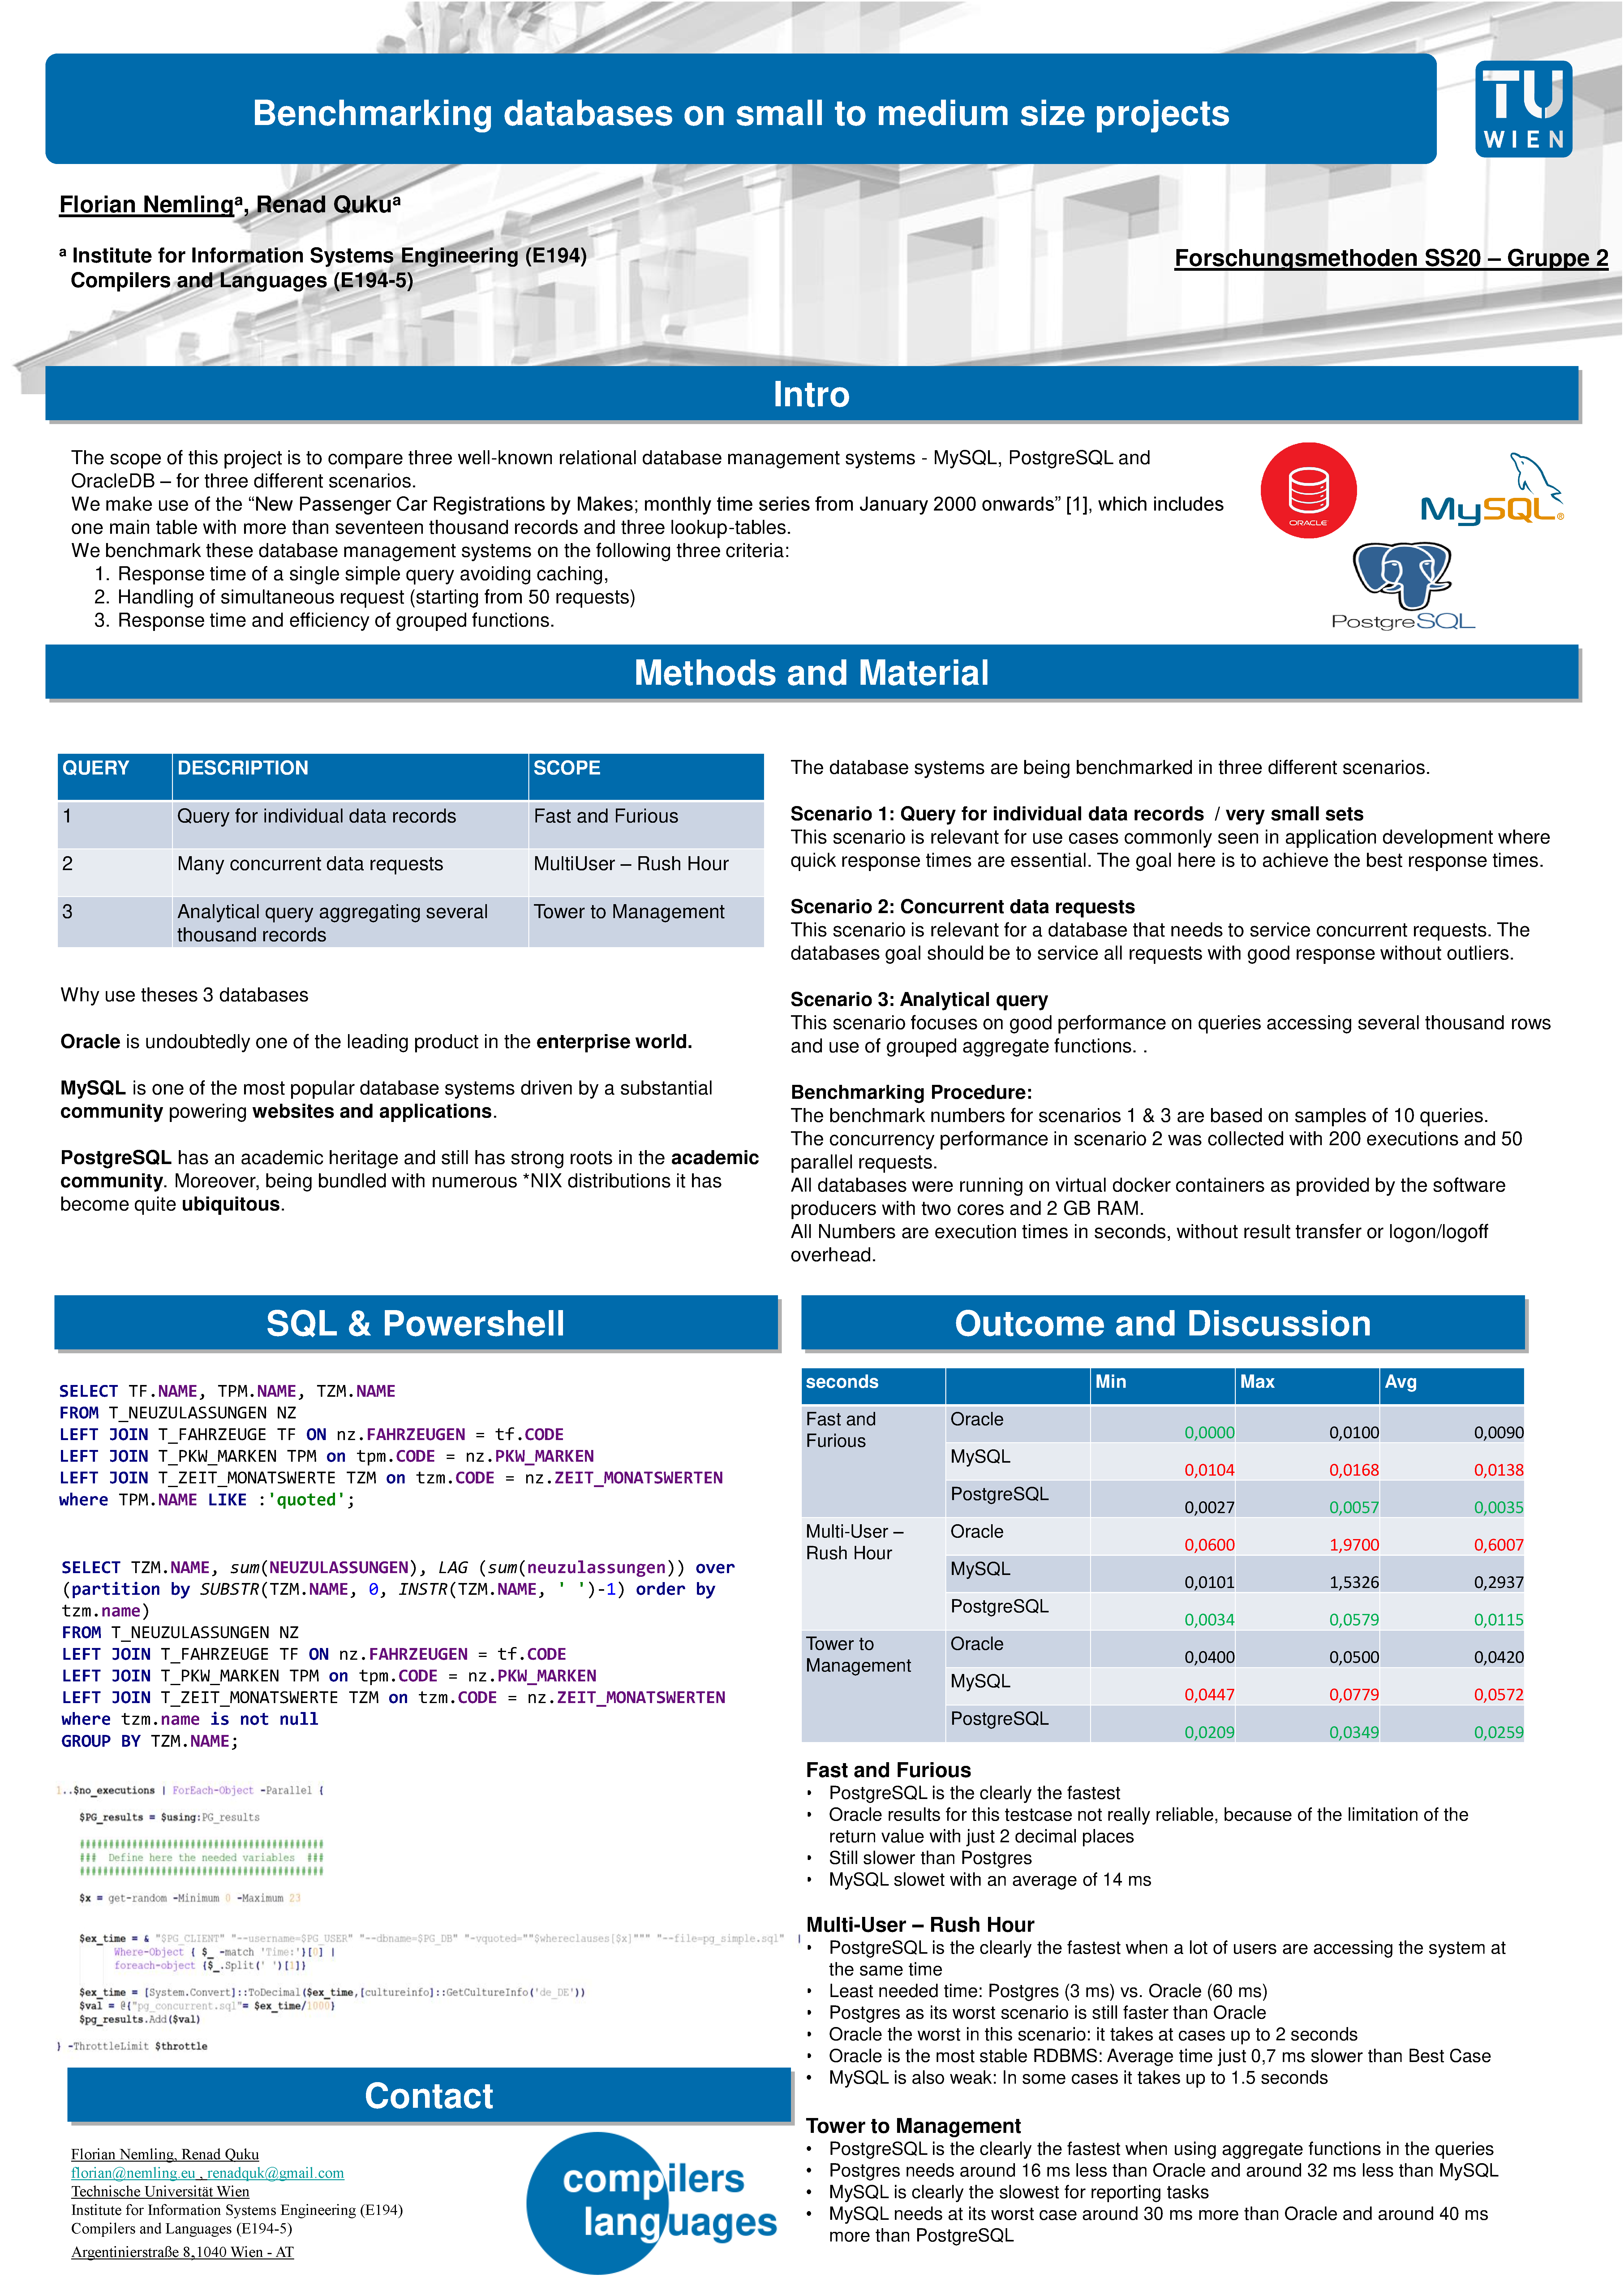
\includepdf[width=\textwidth]{Forschungsmethoden-SS2020-Uebung-2-Gruppe-2.pdf}
\end{document}
